% !TEX program = xelatex

\documentclass{beamer}

\usepackage[utf8]{inputenc}
\usepackage{ctex}

\usepackage{graphicx}
\usepackage{subcaption}

\usepackage{amsmath}
\usepackage{algorithm}
\usepackage{algpseudocode}

\newcommand\norm[1]{\left\lVert#1\right\rVert}


\graphicspath{ {images/} }

%\usetheme{albatross}
\usetheme{Madrid}
\usecolortheme{beaver}
%\usetheme{Antibes}


\title{Sprite sheet的生成 }
\author{卓越羿}
\institute[NUST]{}
\date{2018}

\begin{document}

\frame{\titlepage}

\begin{frame}

\frametitle{Sprite Sheet}

Sprite 是一种游戏或图形应用中2d动画逻辑对象,SpriteSheet则是它的图像素材,
如图 \ref{fig:highpriest} 所示是RPGMaker的一个spritesheet的一部分,表示了
人物的四个方向的行走动作,共3帧。

\begin{figure}[htb]
    \centering
    
\includegraphics[width=0.3\linewidth]{H.png}
    \caption{Spritesheet例子}
    \label{fig:highpriest}
\end{figure}

\end{frame}

\begin{frame}

\frametitle{Live2d e-mote}

从静态单个图片或几个类似的图片中生成动画的技术有e-mote和live2d,相关
作品有有名的nekopara等,它们主要利用一些变形场之类的方法使得角色可以
做出变动不那么大的“动作”,见图 \ref{fig:miku} 

\begin{figure}[htb]
    \centering
    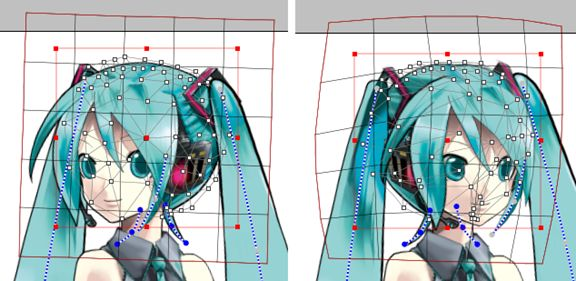
\includegraphics[width=0.7\linewidth]{miku.jpg}
    \caption{变形场}
    \label{fig:miku}
\end{figure}

\end{frame}

\begin{frame}

\frametitle{Delaunay三角形分割映射}

\begin{figure}[htb]
    \centering
    \begin{subfigure}[b]{0.6\linewidth}
        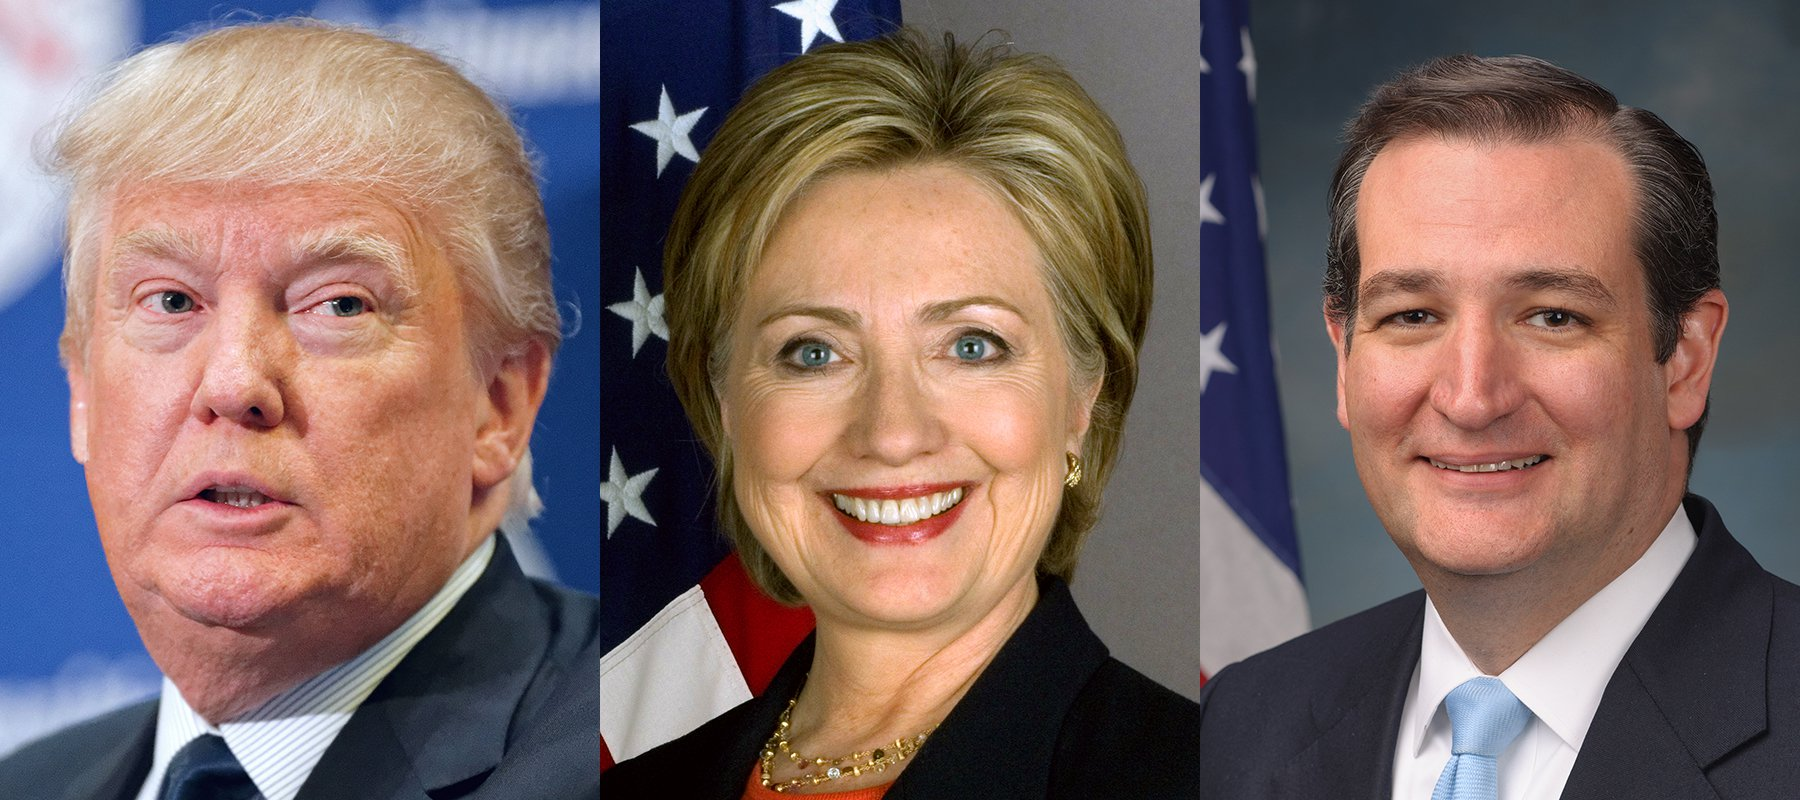
\includegraphics[width=\linewidth]{presidential-original.jpg}
        \caption{原图}
      \end{subfigure}
      \begin{subfigure}[b]{0.6\linewidth}
        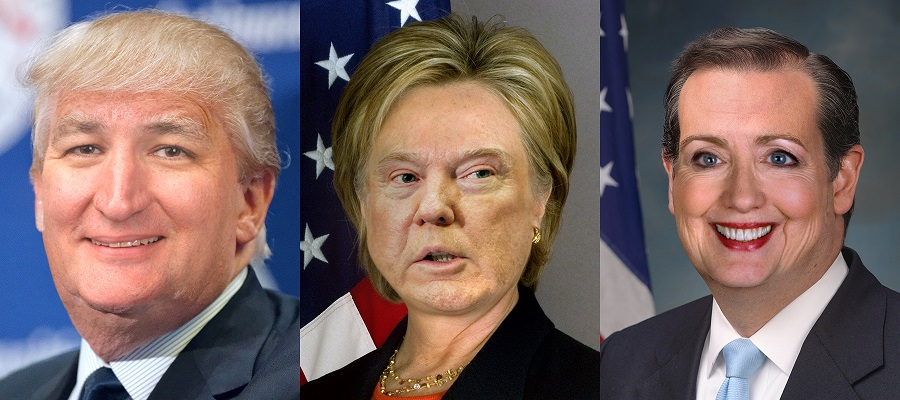
\includegraphics[width=\linewidth]{presidential-swap.jpg}
        \caption{换脸结果}
      \end{subfigure}
      \caption{三个蹩脚竞选人的换脸}
      \label{fig:presid}
\end{figure}

\end{frame}

\begin{frame}

    \frametitle{Delaunay算法}
    
    \begin{algorithm}[H]
        \caption{Delaunay warp}
        \begin{algorithmic}[1]
        \Procedure{Delaunay warp}{img1, img2, points1, points2}
            \State out $\gets$ img2
            \State dt $\gets$ 计算被points对应的的Delaunay三角形
            \For{t in dt}
                \State t1 $\gets$ points1[t]
                \State t2 $\gets$ points2[t]
                \State trans $\gets$ 拟合t1到t2的仿射变换
                \State out $\gets$ trans(out, img1, trans) 
            \EndFor
            \State \textbf{return} out
        \EndProcedure
        \end{algorithmic}
        \label{alg:delwarp}
    \end{algorithm}
    
    \end{frame}

\begin{frame}

\frametitle{Delaunay算法-长者与国王}

\begin{figure}[htb]
    \centering
    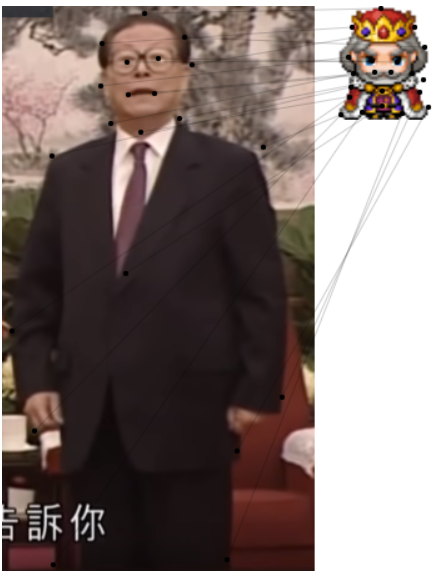
\includegraphics[width=0.4\linewidth]{map.png}
    \caption{长者与国王的关键点对应}
    \label{fig:map}
\end{figure}

\end{frame}

\begin{frame}

\begin{figure}[htb]
    
\includegraphics[width=0.6\linewidth]{tri_elder2king.png}
    \caption{将长者warp为国王}
    \label{fig:elder2king}
\end{figure}

\end{frame}

\begin{frame}

\begin{figure}[htb]
    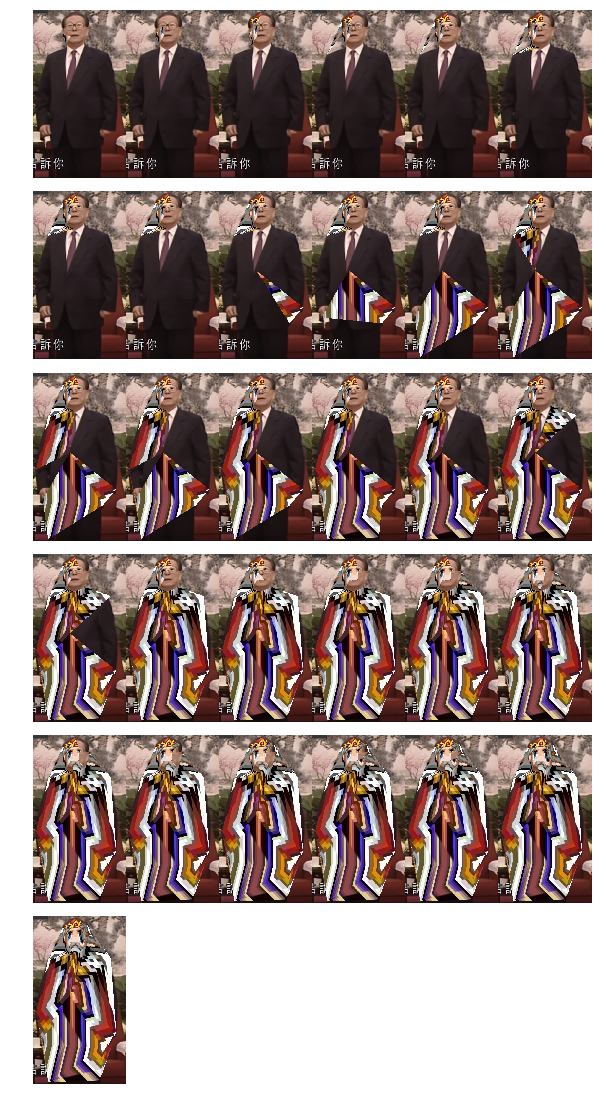
\includegraphics[width=0.3\linewidth]{tri_king2elder.png}
    \caption{将国王warp为长者}
    \label{fig:king2elder}
\end{figure}

\end{frame}

\begin{frame}
\frametitle{正态模型}
收集RPGMaker自带的1332个像素图,拉成向量后求其均值与协方差矩阵
可以得到此类图像分布的多元正态模型,如期望是类似平均脸的东西,如图所示。 

\begin{figure}[htb]
    \centering
    \begin{subfigure}[b]{0.3\linewidth}
        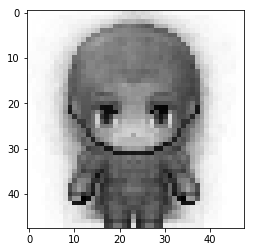
\includegraphics[width=\linewidth]{mean_sprite.png}
        \caption{均值}
      \end{subfigure}
      \begin{subfigure}[b]{0.3\linewidth}
        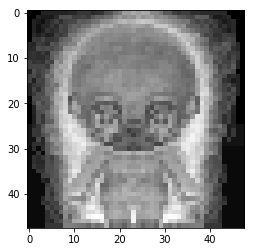
\includegraphics[width=\linewidth]{sd_sprtie.png}
        \caption{标准差}
      \end{subfigure}
      \caption{sprite分布特征}
      \label{fig:meansd}
\end{figure}

\end{frame}

\begin{frame}
\frametitle{直接采样}

形式地,模型为:

$$
X \sim N(\mu, \Sigma) \quad X \in R^d
$$

无论如何设定,多元正态分布可以下式直接采样,协方差矩阵$\Sigma$是实对称矩阵,
所以有cholesky分解,$\Sigma = LL^T$,
从而可通过下式生成$N(\mu,\Sigma)$型随机变量,根据$AX+b \sim N(\mu_X + b, A\Sigma_XA^T)$:

\begin{align*}
    X &\sim N(0, I) \\
    Y &= L X + \mu \sim N(0+\mu,LIL^T) = N(\mu, \Sigma)
\end{align*}


\end{frame}

\begin{frame}
\frametitle{直接采样-结果}

\begin{figure}[htb]
    \centering
    \begin{subfigure}[b]{0.3\linewidth}
        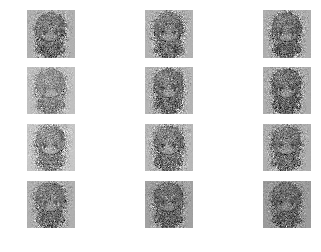
\includegraphics[width=\linewidth]{meanfield.png}
        \caption{meanfield}
      \end{subfigure}
      \begin{subfigure}[b]{0.3\linewidth}
        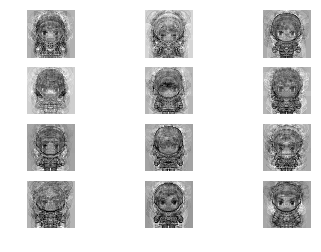
\includegraphics[width=\linewidth]{fullrank.png}
        \caption{fullrank}
      \end{subfigure}
      \caption{正态模型直接采样}
      \label{fig:meanfieldfullrank}
\end{figure}

\end{frame}

\begin{frame}
\frametitle{条件采样}
利用多元正态分布的条件分布关系:

\begin{align*}
    (x_1 \, x_2) &\sim N((\mu_1,\mu_2),\Sigma) \\ 
    x_1 \mid x_2 = a &\sim N(\bar{\mu},\bar{\Sigma}) \\
    \bar{\mu} &= \mu_1 + \Sigma_{12}\Sigma^{-1}_{22}(a - \mu_2) \\
    \bar{\Sigma} &= \Sigma_{11} - \Sigma_{12}\Sigma_{22}^{-1}\Sigma_{21}
\end{align*}

可以进行条件采样
    
\end{frame}

\begin{frame}
下面将6个没有列入训练集的样本分别把上半部下半部分左半部分右半部分遮住,
用没遮住的另一边去计算其条件分布进行采样。

\begin{figure}[htb]
    \centering
    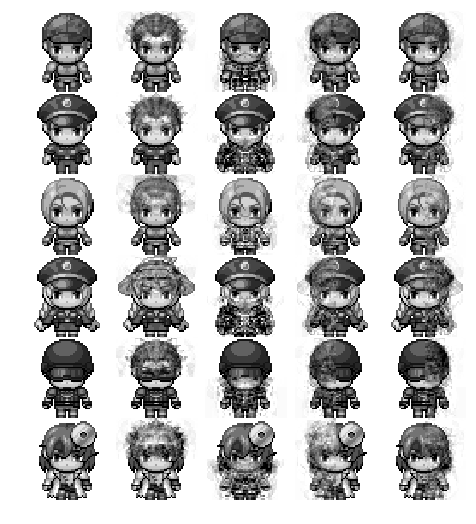
\includegraphics[width=0.6\linewidth]{normal_conditional_sample.png}
    \caption{正态条件采样,测试集}
    \label{fig:normcond1}
  \end{figure}
\end{frame}

\begin{frame}
\frametitle{不同分布数据的采样}

\begin{figure}[htb]
    \centering
      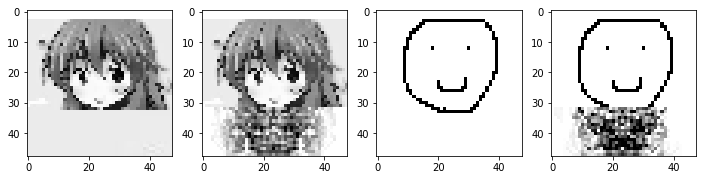
\includegraphics[width=\linewidth]{normal_real_test.png}
      \caption{HP和火柴人的正态模型条件推断}
      \label{fig:normalreal}
  \end{figure}
硬模板方法果然不可能成功
\end{frame}

\begin{frame}
\frametitle{CycleGAN}

CycleGAN \cite{zhu2017unpaired} 提供了一种无监督的将两个图像域中的图像转换的方法,如将马换成斑马或者狗变猫等。

它由四个网络构成,GA,GB,DA,DB,GA试图将A域图片转成B域图片,GB则试图将B域图片转为A域图片。DA,DB则鉴别一个图片
是来自真实分布$p_{data}(x)$还是来自由GA,GB定义的隐式分布$GA(y) \quad y \sim p_{data}(y)$。

数据集如下:

\begin{figure}[htb]
    \centering
    \begin{subfigure}[b]{0.2\linewidth}
        
\includegraphics[width=\linewidth]{hp.jpg}
        \caption{A域}
      \end{subfigure}
      \begin{subfigure}[b]{0.2\linewidth}
        
\includegraphics[width=\linewidth]{bigsprite.png}
        \caption{B域}
      \end{subfigure}
      \caption{CycleGAN数据集}
      \label{fig:hp2sprite}
\end{figure}

\end{frame}

\begin{frame}
\frametitle{Loss定义}
\begin{align*}
    \mathcal{L}(G,D) &= \mathcal{L}_{GAN}(G_A,D_B) \\
                                    &+ \mathcal{L}_{GAN}(G_B,D_A) \\
                                    &+ \lambda \mathcal{L}_{cyc}(G_A,G_B) + \gamma \mathcal{L}_{iden}(G_A,G_B) \\
        \mathcal{L}_{GAN}(G_X,D_Y) &= \mathbb{E}_{y\sim p_{data}(y)}(\log D_Y(y))  \\
                                    &+ \mathbb{E}_{x \sim p_{data}(x)} \log(1-D_Y(G(x)))  \\
        \mathcal{L}_{cyc}(G_A,G_B) &= \mathbb{E}_{x\sim p_{data}(x)} (\norm{G_B(G_A(x)) - x}_1) \\
                                    &+ \mathbb{E}_{y\sim p_{data}(y)} (\norm{G_A(G_B(y)) - y}_1) \\
        \mathcal{L}_{iden}(G_A,G_B) &= \mathbb{E}_{y \sim p_{data}(y)}(\norm{G_B(y)-y}_1) \\
                                    &+ \mathbb{E}_{x \sim p_{data}(x)}(\norm{G_A(x)-x}_1)
    \end{align*}
        
\end{frame}

\begin{frame}
其中$\mathcal{L}_{GAN}(G_X,D_Y)(X,Y \in \{A,B\})$定义了$A \to B$与$B \to A$的GAN损失,也就是将来自A域样本判成由B域经$G_B$生成的
假A样本与将假A样本判成真A样本均带来损失。这个损失是对$D_A,D_B$来说的。对$G_A,G_B$,可以看作把真实样本判成错的损失拿掉,
因为$G_X$的参数本身也不能控制这个错误,而把把将它生成的错判伪造样本取负,即向鼓励$D_X$错判的方向优化。

循环损失$\mathcal{L}_{cyc}(G_A,G_B)$约束网络应该应当在将一个A域的图由$G_A$变为B域的图后,
再由$G_B$变回来时大致相同。可看成一种正则项,但实际训练时会发现有时由于$D_X$过于强大,主要目标$\mathcal{L}_{GAN}$
在小参数变化下没什么起色,结果算法就一股劲去优化这个循环损失了,反而加剧了GAN训练死亡困境。

恒等映射损失$\mathcal{L}_{iden}$要求B域图片经过$G_A$映射($G_A$本身被要求把$A$域的图片映射到$B$域)应该没有变化。
这个损失在原文\cite{zhu2017unpaired}是个可选的正则项,也有之前提到的问题。另外这个项的引入使得默认了两个域的图像
尺寸一样,而我的问题里两个域的图像尺寸是不一样的,所以我分别用了把两个域的图片转成一样的与改变这个损失的定义的方法。

分类器$D_X$与生成器$G_X$对每个样本各训练一次为一个epoch,有时考虑分类器过于强大也考虑让生成器多训练几个step或者
调大学习率,不过感觉效果不明显。
    
\end{frame}

\begin{frame}
\frametitle{实验一}
网络结构与 \cite{zhu2017unpaired}的基线实现完全一致,
其中GA(B)就是resnet\_9blocks的实现,结构为:c7s1-64,d128,d256,R256,R256,R256,R256,
R256,R256,R256,R256,R256,u128,u64,c7s1-3。DA(B)的网络结构也完全一致,也就是 C64-C128-C256-C512。
结果如图所示

\begin{figure}[htb]
    \centering
    \begin{subfigure}[b]{0.24\linewidth}
        
\includegraphics[width=\linewidth]{NSFW.png}
        \caption{$x \in A$}
      \end{subfigure}
      \begin{subfigure}[b]{0.24\linewidth}
        
\includegraphics[width=\linewidth]{exp1_fake_B.png}
        \caption{$G_A(x)$}
      \end{subfigure}
      \begin{subfigure}[b]{0.24\linewidth}
        
\includegraphics[width=\linewidth]{exp1_real_B.png}
        \caption{$y \in B$}
      \end{subfigure}
      \begin{subfigure}[b]{0.24\linewidth}
        
\includegraphics[width=\linewidth]{exp1_fake_A.png}
        \caption{$G_B(y)$}
      \end{subfigure}
      \caption{实验1结果}
      \label{fig:exp1}
\end{figure}
\end{frame}

\begin{frame}
\frametitle{实验二}
去掉了$100 \times 100 \to 64 \times 64$的random crop。
\begin{figure}[htb]
    \centering
    \begin{subfigure}[b]{0.23\linewidth}
        
\includegraphics[width=\linewidth]{exp2_epoch004_real_A.png}
        \caption{$x \in A$}
      \end{subfigure}
      \begin{subfigure}[b]{0.23\linewidth}
        
\includegraphics[width=\linewidth]{exp2_epoch004_fake_B.png}
        \caption{$G_A(x)$}
      \end{subfigure}
      \begin{subfigure}[b]{0.23\linewidth}
        
\includegraphics[width=\linewidth]{exp2_epoch004_rec_A.png}
        %\caption{$G_B(G_A(x))$}
        \caption{$G_{BA}(x))$}
      \end{subfigure}
      \begin{subfigure}[b]{0.23\linewidth}
        
\includegraphics[width=\linewidth]{exp2_epoch004_idt_A.png}
        \caption{$G_A(y)$}
      \end{subfigure}
      \begin{subfigure}[b]{0.23\linewidth}
        
\includegraphics[width=\linewidth]{exp2_epoch004_real_B.png}
        \caption{$y \in B$}
      \end{subfigure}
      \begin{subfigure}[b]{0.23\linewidth}
        
\includegraphics[width=\linewidth]{exp2_epoch004_fake_A.png}
        \caption{$G_B(y)$}
      \end{subfigure}
      \begin{subfigure}[b]{0.23\linewidth}
        
\includegraphics[width=\linewidth]{exp2_epoch004_rec_B.png}
        %\caption{$G_A(G_B(y))$}
        \caption{$G_{AB}(y))$}
      \end{subfigure}
      \begin{subfigure}[b]{0.23\linewidth}
        
\includegraphics[width=\linewidth]{exp2_epoch004_idt_B.png}
        \caption{$G_B(x)$}
      \end{subfigure}
      \caption{实验2epoch4的结果}
      \label{fig:exp2epoch4}
\end{figure}

\end{frame}

\begin{frame}
开始训练进行的还行。
\begin{figure}[htb]
    \centering
    \begin{subfigure}[b]{0.23\linewidth}
        
\includegraphics[width=\linewidth]{exp2_epoch060_real_A.png}
        \caption{$x \in A$}
      \end{subfigure}
      \begin{subfigure}[b]{0.23\linewidth}
        
\includegraphics[width=\linewidth]{exp2_epoch060_fake_B.png}
        \caption{$G_A(x)$}
      \end{subfigure}
      \begin{subfigure}[b]{0.23\linewidth}
        
\includegraphics[width=\linewidth]{exp2_epoch060_rec_A.png}
        %\caption{$G_B(G_A(x))$}
        \caption{$G_{BA}(x))$}
      \end{subfigure}
      \begin{subfigure}[b]{0.23\linewidth}
        
\includegraphics[width=\linewidth]{exp2_epoch060_idt_A.png}
        \caption{$G_A(y)$}
      \end{subfigure}
      \begin{subfigure}[b]{0.23\linewidth}
        
\includegraphics[width=\linewidth]{exp2_epoch060_real_B.png}
        \caption{$y \in B$}
      \end{subfigure}
      \begin{subfigure}[b]{0.23\linewidth}
        
\includegraphics[width=\linewidth]{exp2_epoch060_fake_A.png}
        \caption{$G_B(y)$}
      \end{subfigure}
      \begin{subfigure}[b]{0.23\linewidth}
        
\includegraphics[width=\linewidth]{exp2_epoch060_rec_B.png}
        %\caption{$G_A(G_B(y))$}
        \caption{$G_{AB}(y))$}
      \end{subfigure}
      \begin{subfigure}[b]{0.23\linewidth}
        
\includegraphics[width=\linewidth]{exp2_epoch060_idt_B.png}
        \caption{$G_B(x)$}
      \end{subfigure}
      \caption{实验2epoch60的结果}
      \label{fig:exp2epoch60}
\end{figure}

\end{frame}
\begin{frame}
然后突然崩了,$G_A(x)$沉迷于优化另外两个loss。
\begin{figure}[htb]
    \centering
    \begin{subfigure}[b]{0.23\linewidth}
        
\includegraphics[width=\linewidth]{exp2_epoch100_real_A.png}
        \caption{$x \in A$}
      \end{subfigure}
      \begin{subfigure}[b]{0.23\linewidth}
        
\includegraphics[width=\linewidth]{exp2_epoch100_fake_B.png}
        \caption{$G_A(x)$}
      \end{subfigure}
      \begin{subfigure}[b]{0.23\linewidth}
        
\includegraphics[width=\linewidth]{exp2_epoch100_rec_A.png}
        %\caption{$G_B(G_A(x))$}
        \caption{$G_{BA}(x))$}
      \end{subfigure}
      \begin{subfigure}[b]{0.23\linewidth}
        
\includegraphics[width=\linewidth]{exp2_epoch100_idt_A.png}
        \caption{$G_A(y)$}
      \end{subfigure}
      \begin{subfigure}[b]{0.23\linewidth}
        
\includegraphics[width=\linewidth]{exp2_epoch100_real_B.png}
        \caption{$y \in B$}
      \end{subfigure}
      \begin{subfigure}[b]{0.23\linewidth}
        
\includegraphics[width=\linewidth]{exp2_epoch100_fake_A.png}
        \caption{$G_B(y)$}
      \end{subfigure}
      \begin{subfigure}[b]{0.23\linewidth}
        
\includegraphics[width=\linewidth]{exp2_epoch100_rec_B.png}
        %\caption{$G_A(G_B(y))$}
        \caption{$G_{AB}(y))$}
      \end{subfigure}
      \begin{subfigure}[b]{0.23\linewidth}
        
\includegraphics[width=\linewidth]{exp2_epoch100_idt_B.png}
        \caption{$G_B(x)$}
      \end{subfigure}
      \caption{实验2epoch100的结果}
      \label{fig:exp2epoch100}
\end{figure}

\end{frame}

\begin{frame}
    从loss曲线可以观察到epoch 96附近的突变,与优化重心的转移。
    \begin{figure}[htb]
        \centering
        \begin{subfigure}[b]{0.23\linewidth}
            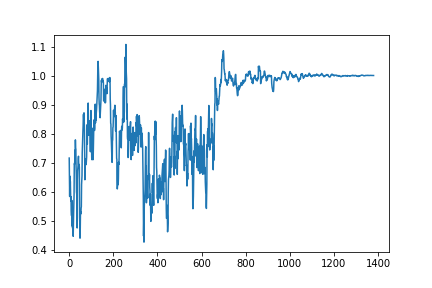
\includegraphics[width=\linewidth]{exp2_G_A.png}
            \caption{$\mathcal{L}_{G_A}$}
          \end{subfigure}
          \begin{subfigure}[b]{0.23\linewidth}
            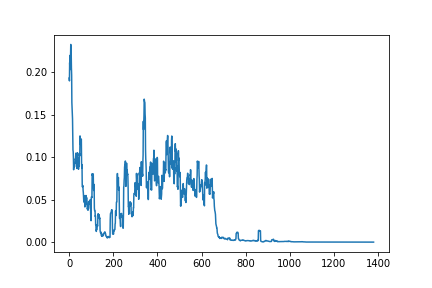
\includegraphics[width=\linewidth]{exp2_D_A.png}
            \caption{$\mathcal{L}_{D_A}$}
          \end{subfigure}
          \begin{subfigure}[b]{0.23\linewidth}
            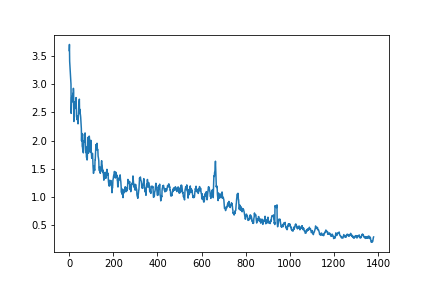
\includegraphics[width=\linewidth]{exp2_cycle_A.png}
            %\caption{$G_B(G_A(x))$}
            \caption{$\mathcal{L}_{cycle,A}$}
          \end{subfigure}
          \begin{subfigure}[b]{0.23\linewidth}
            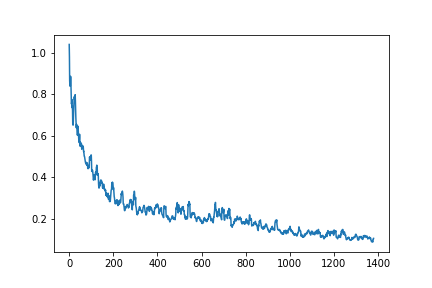
\includegraphics[width=\linewidth]{exp2_idt_A.png}
            \caption{$\mathcal{L}_{iden,A}$}
          \end{subfigure}
          \begin{subfigure}[b]{0.23\linewidth}
            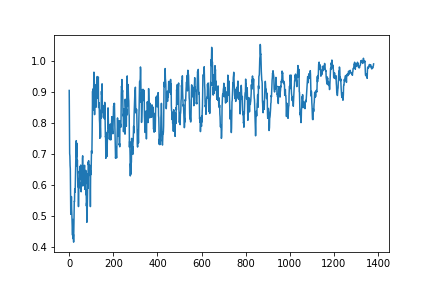
\includegraphics[width=\linewidth]{exp2_G_B.png}
            \caption{$\mathcal{L}_{G_B}$}
          \end{subfigure}
          \begin{subfigure}[b]{0.23\linewidth}
            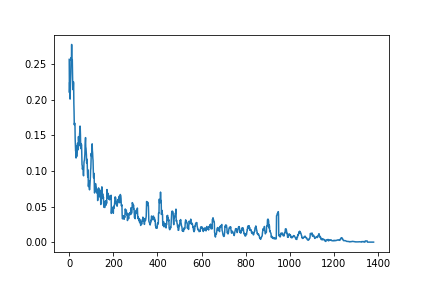
\includegraphics[width=\linewidth]{exp2_D_B.png}
            \caption{$\mathcal{L}_{D_B}$}
          \end{subfigure}
          \begin{subfigure}[b]{0.23\linewidth}
            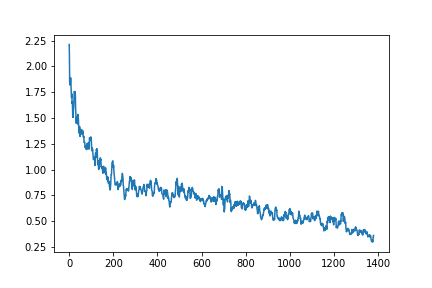
\includegraphics[width=\linewidth]{exp2_cycle_B.png}
            %\caption{$G_B(G_A(x))$}
            \caption{$\mathcal{L}_{cycle,B}$}
          \end{subfigure}
          \begin{subfigure}[b]{0.23\linewidth}
            \includegraphics[width=\linewidth]{exp2_idt_B.png}
            \caption{$\mathcal{L}_{iden,B}$}
          \end{subfigure}
          \caption{实验2 loss曲线}
          \label{fig:exp2loss}
    \end{figure}
\end{frame}

\begin{frame}
\frametitle{实验三}
从实验二epoch 90的快照重新开始训练

\begin{figure}[htb]
    \centering
    \begin{subfigure}[b]{0.23\linewidth}
        \includegraphics[width=\linewidth]{exp3_epoch194_real_A.png}
        \caption{$x \in A$}
      \end{subfigure}
      \begin{subfigure}[b]{0.23\linewidth}
        \includegraphics[width=\linewidth]{exp3_epoch194_fake_B.png}
        \caption{$G_A(x)$}
      \end{subfigure}
      \begin{subfigure}[b]{0.23\linewidth}
        \includegraphics[width=\linewidth]{exp3_epoch194_rec_A.png}
        %\caption{$G_B(G_A(x))$}
        \caption{$G_{BA}(x))$}
      \end{subfigure}
      \begin{subfigure}[b]{0.23\linewidth}
        \includegraphics[width=\linewidth]{exp3_epoch194_idt_A.png}
        \caption{$G_A(y)$}
      \end{subfigure}
      \begin{subfigure}[b]{0.23\linewidth}
        \includegraphics[width=\linewidth]{exp3_epoch194_real_B.png}
        \caption{$y \in B$}
      \end{subfigure}
      \begin{subfigure}[b]{0.23\linewidth}
        \includegraphics[width=\linewidth]{exp3_epoch194_fake_A.png}
        \caption{$G_B(y)$}
      \end{subfigure}
      \begin{subfigure}[b]{0.23\linewidth}
        \includegraphics[width=\linewidth]{exp3_epoch194_rec_B.png}
        %\caption{$G_A(G_B(y))$}
        \caption{$G_{AB}(y))$}
      \end{subfigure}
      \begin{subfigure}[b]{0.23\linewidth}
        \includegraphics[width=\linewidth]{exp3_epoch194_idt_B.png}
        \caption{$G_B(x)$}
      \end{subfigure}
      \caption{实验3 epoch194的结果}
      \label{fig:exp3epoch194}
\end{figure}

\end{frame}

\begin{frame}
这一次没什么变化却没有出现崩坏现象。
\begin{figure}[htb]
    \centering
    \begin{subfigure}[b]{0.23\linewidth}
        \includegraphics[width=\linewidth]{exp3_G_A.png}
        \caption{$\mathcal{L}_{G_A}$}
      \end{subfigure}
      \begin{subfigure}[b]{0.23\linewidth}
        \includegraphics[width=\linewidth]{exp3_D_A.png}
        \caption{$\mathcal{L}_{D_A}$}
      \end{subfigure}
      \begin{subfigure}[b]{0.23\linewidth}
        \includegraphics[width=\linewidth]{exp3_cycle_A.png}
        %\caption{$G_B(G_A(x))$}
        \caption{$\mathcal{L}_{cycle,A}$}
      \end{subfigure}
      \begin{subfigure}[b]{0.23\linewidth}
        \includegraphics[width=\linewidth]{exp3_idt_A.png}
        \caption{$\mathcal{L}_{iden,A}$}
      \end{subfigure}
      \begin{subfigure}[b]{0.23\linewidth}
        \includegraphics[width=\linewidth]{exp3_G_B.png}
        \caption{$\mathcal{L}_{G_B}$}
      \end{subfigure}
      \begin{subfigure}[b]{0.23\linewidth}
        \includegraphics[width=\linewidth]{exp3_D_B.png}
        \caption{$\mathcal{L}_{D_B}$}
      \end{subfigure}
      \begin{subfigure}[b]{0.23\linewidth}
        \includegraphics[width=\linewidth]{exp3_cycle_B.png}
        %\caption{$G_B(G_A(x))$}
        \caption{$\mathcal{L}_{cycle,B}$}
      \end{subfigure}
      \begin{subfigure}[b]{0.23\linewidth}
        \includegraphics[width=\linewidth]{exp3_idt_B.png}
        \caption{$\mathcal{L}_{iden,B}$}
      \end{subfigure}
      \caption{实验3 loss曲线}
      \label{fig:exp3loss}
\end{figure}
\end{frame}

\begin{frame}
\frametitle{实验四}
$\mathcal{L}_{iden}$的权重从$0.5$调到$1.0$
\begin{figure}[htb]
    \centering
    \begin{subfigure}[b]{0.23\linewidth}
        \includegraphics[width=\linewidth]{exp4_G_A.png}
        \caption{$\mathcal{L}_{G_A}$}
      \end{subfigure}
      \begin{subfigure}[b]{0.23\linewidth}
        \includegraphics[width=\linewidth]{exp4_D_A.png}
        \caption{$\mathcal{L}_{D_A}$}
      \end{subfigure}
      \begin{subfigure}[b]{0.23\linewidth}
        \includegraphics[width=\linewidth]{exp4_cycle_A.png}
        %\caption{$G_B(G_A(x))$}
        \caption{$\mathcal{L}_{cycle,A}$}
      \end{subfigure}
      \begin{subfigure}[b]{0.23\linewidth}
        \includegraphics[width=\linewidth]{exp4_idt_A.png}
        \caption{$\mathcal{L}_{iden,A}$}
      \end{subfigure}
      \begin{subfigure}[b]{0.23\linewidth}
        \includegraphics[width=\linewidth]{exp4_G_B.png}
        \caption{$\mathcal{L}_{G_B}$}
      \end{subfigure}
      \begin{subfigure}[b]{0.23\linewidth}
        \includegraphics[width=\linewidth]{exp4_D_B.png}
        \caption{$\mathcal{L}_{D_B}$}
      \end{subfigure}
      \begin{subfigure}[b]{0.23\linewidth}
        \includegraphics[width=\linewidth]{exp4_cycle_B.png}
        %\caption{$G_B(G_A(x))$}
        \caption{$\mathcal{L}_{cycle,B}$}
      \end{subfigure}
      \begin{subfigure}[b]{0.23\linewidth}
        \includegraphics[width=\linewidth]{exp4_idt_B.png}
        \caption{$\mathcal{L}_{iden,B}$}
      \end{subfigure}
      \caption{实验4 loss曲线}
      \label{fig:exp3loss}
\end{figure}
\end{frame}

\begin{frame}
\frametitle{实验五}
生成器仅使用6个residual block
\begin{figure}[htb]
    \centering
    \begin{subfigure}[b]{0.23\linewidth}
        \includegraphics[width=\linewidth]{exp5_epoch140_real_A.png}
        \caption{$x \in A$}
      \end{subfigure}
      \begin{subfigure}[b]{0.23\linewidth}
        \includegraphics[width=\linewidth]{exp5_epoch140_fake_B.png}
        \caption{$G_A(x)$}
      \end{subfigure}
      \begin{subfigure}[b]{0.23\linewidth}
        \includegraphics[width=\linewidth]{exp5_epoch140_rec_A.png}
        %\caption{$G_B(G_A(x))$}
        \caption{$G_{BA}(x))$}
      \end{subfigure}
      \begin{subfigure}[b]{0.23\linewidth}
        \includegraphics[width=\linewidth]{exp5_epoch140_idt_A.png}
        \caption{$G_A(y)$}
      \end{subfigure}
      \begin{subfigure}[b]{0.23\linewidth}
        \includegraphics[width=\linewidth]{exp5_epoch140_real_B.png}
        \caption{$y \in B$}
      \end{subfigure}
      \begin{subfigure}[b]{0.23\linewidth}
        \includegraphics[width=\linewidth]{exp5_epoch140_fake_A.png}
        \caption{$G_B(y)$}
      \end{subfigure}
      \begin{subfigure}[b]{0.23\linewidth}
        \includegraphics[width=\linewidth]{exp5_epoch140_rec_B.png}
        %\caption{$G_A(G_B(y))$}
        \caption{$G_{AB}(y))$}
      \end{subfigure}
      \begin{subfigure}[b]{0.23\linewidth}
        \includegraphics[width=\linewidth]{exp5_epoch140_idt_B.png}
        \caption{$G_B(x)$}
      \end{subfigure}
      \caption{实验5 epoch140的结果}
      \label{fig:exp5epoch140}
\end{figure}
\end{frame}


\begin{frame}
\frametitle{实验六}
同实验五设计,但给$\mathcal{L}_{GAN}$的损失权重加一倍
\begin{figure}[htb]
    \centering
    \begin{subfigure}[b]{0.23\linewidth}
        \includegraphics[width=\linewidth]{exp6_G_A.png}
        \caption{$\mathcal{L}_{G_A}$}
      \end{subfigure}
      \begin{subfigure}[b]{0.23\linewidth}
        \includegraphics[width=\linewidth]{exp6_D_A.png}
        \caption{$\mathcal{L}_{D_A}$}
      \end{subfigure}
      \begin{subfigure}[b]{0.23\linewidth}
        \includegraphics[width=\linewidth]{exp6_cycle_A.png}
        %\caption{$G_B(G_A(x))$}
        \caption{$\mathcal{L}_{cycle,A}$}
      \end{subfigure}
      \begin{subfigure}[b]{0.23\linewidth}
        \includegraphics[width=\linewidth]{exp6_idt_A.png}
        \caption{$\mathcal{L}_{iden,A}$}
      \end{subfigure}
      \begin{subfigure}[b]{0.23\linewidth}
        \includegraphics[width=\linewidth]{exp6_G_B.png}
        \caption{$\mathcal{L}_{G_B}$}
      \end{subfigure}
      \begin{subfigure}[b]{0.23\linewidth}
        \includegraphics[width=\linewidth]{exp6_D_B.png}
        \caption{$\mathcal{L}_{D_B}$}
      \end{subfigure}
      \begin{subfigure}[b]{0.23\linewidth}
        \includegraphics[width=\linewidth]{exp6_cycle_B.png}
        %\caption{$G_B(G_A(x))$}
        \caption{$\mathcal{L}_{cycle,B}$}
      \end{subfigure}
      \begin{subfigure}[b]{0.23\linewidth}
        \includegraphics[width=\linewidth]{exp6_idt_B.png}
        \caption{$\mathcal{L}_{iden,B}$}
      \end{subfigure}
      \caption{实验5,6 loss曲线}
      \label{fig:exp6loss}
\end{figure}   
\end{frame}


\begin{frame}
\frametitle{实验七}

之前的实验中均采取将两域图片压成同尺寸处理的方法,如果A域图片作为本来的大尺寸高分辨率的图片保持相对较多的信息
($192/times 192$,取$192$是因为注意到$48$放大4倍后为$192$
)而B域图片不进行蹩脚的升采样(保持$48\times 48$而非$64\times 64$),结果是否会有改善呢?直接
修改输入输出是不可行的,因为$\mathcal{L}_{iden}$要求两域相同,一种方式是直接取消这个项,不过我是直接线性插值。
而且此时两个生成器的结构是不一样的。$G_A$为c7s1-32,d64,d128,R128x6,c7s1-3。即去掉将尺寸增大(恢复)的层,同时
隐单元数全体除以2,由于显存的原因
而$G_B$类似,为:c7s1-32,R128x6,u128,u64,c7s1-3。即去掉了降尺寸的层,同时单元数减一半。而判别器与之前结构类似,
但单元数除以4以令两者的能力差不那么大以期能够改善优化。

\end{frame}
\begin{frame}
    然而并没有什么改善。
\begin{figure}[htb]
    \centering
    \begin{subfigure}[b]{0.23\linewidth}
        \includegraphics[width=\linewidth]{exp7_epoch061_real_A.png}
        \caption{$x \in A$}
      \end{subfigure}
      \begin{subfigure}[b]{0.23\linewidth}
        \includegraphics[width=\linewidth]{exp7_epoch061_fake_B.png}
        \caption{$G_A(x)$}
      \end{subfigure}
      \begin{subfigure}[b]{0.23\linewidth}
        \includegraphics[width=\linewidth]{exp7_epoch061_rec_A.png}
        %\caption{$G_B(G_A(x))$}
        \caption{$G_{BA}(x))$}
      \end{subfigure}
      \begin{subfigure}[b]{0.23\linewidth}
        \includegraphics[width=\linewidth]{exp7_epoch061_idt_A.png}
        \caption{$G_A(y)$}
      \end{subfigure}
      \begin{subfigure}[b]{0.23\linewidth}
        \includegraphics[width=\linewidth]{exp7_epoch061_real_B.png}
        \caption{$y \in B$}
      \end{subfigure}
      \begin{subfigure}[b]{0.23\linewidth}
        \includegraphics[width=\linewidth]{exp7_epoch061_fake_A.png}
        \caption{$G_B(y)$}
      \end{subfigure}
      \begin{subfigure}[b]{0.23\linewidth}
        \includegraphics[width=\linewidth]{exp7_epoch061_rec_B.png}
        %\caption{$G_A(G_B(y))$}
        \caption{$G_{AB}(y))$}
      \end{subfigure}
      \begin{subfigure}[b]{0.23\linewidth}
        \includegraphics[width=\linewidth]{exp7_epoch061_idt_B.png}
        \caption{$G_B(x)$}
      \end{subfigure}
      \caption{实验7 epoch61的结果}
      \label{fig:exp7epoch61}
\end{figure}
\end{frame}

\begin{frame}
很惭愧,只做了三个微小的方法。

\begin{figure}[htb]
    \includegraphics[width=0.9\linewidth]{elder.png}
\end{figure}
    
\end{frame}

\end{document}